\documentclass[10pt,norsk,a4paper]{article}
\usepackage[utf8]{inputenc}
\usepackage[T1]{fontenc}
\usepackage[norsk]{babel}
% - PDF-relatert
\usepackage{hyperref,pdfpages,hypcap}
\hypersetup{colorlinks=true,allcolors=.}
\newcommand\fhref[2]{%
	\href{#1}{#2}\footnote{\url{#1}}%
}
% Andre pakker
\usepackage[cm]{fullpage}
\usepackage{parskip,multicol,textcomp,amssymb,graphicx,color,enumitem}
% - Korreksjon av fotnoter i seksjoner/overskrifter
\usepackage[stable]{footmisc}
% - Skrifttype
\usepackage[bitstream-charter]{mathdesign}
% - Kommentarer
\usepackage{comment}


\title{Generalforsamling \\
	Høsten 2018\\[3cm]
	
\includegraphics[width=0.5\textwidth]{cyb-logo.eps}\\[-.5cm]}
\date{14.\ november 2018}
\author{Cybernetisk Selskab}

% Blank header, samt footer med side x av y
\usepackage{fancyhdr}
\pagestyle{fancy}
\renewcommand{\headrulewidth}{0pt}
\fancyhead{}
\cfoot{Side~\thepage\ av~\pageref*{lastpage}}


\begin{document}

\maketitle{}
\newpage
\tableofcontents

\part*{Agenda}

\section{Valg av møteleder}

\section{Valg av referent}

\section{Valg av protokollunderskrivere}

\section{Valg av tellekorps}

\section{Godkjenning av innkalling}

\section{Godkjenning av dagsorden}

%\newpage

\section{Semesterberetninger}
\subsection{Semesterberetning ved leder}

Hei til deg, CYB-er og bidragsyter,

\begin{multicols}{2}
Takk for at du er her. Generalforsamlingen er foreningens øverste organ, og det er utrolig fint at du tar turen innom. Om du er ekstra heldig har du et medlemskap, og sitter derfor med både dagsorden og din stemmeseddel i hånden. Du er med andre ord --- forhåpentligvis --- klar for generalforsamlingen. Om du mot formodning ikke har tatt en stol ennå kan det være lurt. Den blir nok litt varm i løpet av de (korte!) timene du og vi skal tilbringe i formell saksgangs ære og, beklageligvis, tidvis frustrasjon.

Det har et vært et semester som har gitt oss muligheten til å vokse internt. Og det har vi.

I motsetning til det du ser rundt deg akkurat nå --- et levende liv av forberedelser, smålig panikk, kanskje en altfor stor logo projisert på et lerret eller nærmest komplett ro --- har det vært et litt stille hovedstyre utad i foreningen. Vi har blitt utfordret på hva vi mener, og vi har måtte ta vanskelige valg. Utfordringer og vanskelige valg er vel og bra, men arbeid som foregår i kulissene er ikke like så. Samtidig har en delvis innsats blitt gjort for å bedre åpenheten. Vår interne wiki blir gradvis flyttet ut til en åpen wiki, med hjelp fra styremedlemmer, interne og arkivar. Her er det mye papir som må tygges, og om nettopp du liker sånt er det bare å ta kontakt med oss. Mer åpenhet er viktig både for internmassen, men også for de andre foreningene og medlemmene ellers på instituttet som lett ser på CYB og Escape som en \textit{black box}. Grensesnittet vårt er greit definert, men hvordan i alle dager implementasjonen ser ut forblir et mysterium for altfor mange.

Det er mange prosjekter som svever i luften. Alle de ønsker vi å gjøre synlig for internmassen, og vi ønsker å invitere nettopp deg til å bidra her skulle du ønske det. Du har nettopp den muligheten til å forme foreningen \textit{uten} å måtte være i et styreverv, \textit{uten} å måtte være en gruppeleder --- \textit{uten} å ta på deg mer tid enn det du har å gi. Eksempler er slike prosjekter og problemstillinger som GDPR:\@ det kom og forble, og selv om en del kartlegging er påbegynt er det fortsatt mye som gjenstår. Andre prosjekter inkluderer mer en delvis omstilling for å gi mer autonomi til arbeidsgrupper, og mer ansvar.

Man finner raskt andre arenaer hvor man er sårt klar over vårt ansvar og manglende rammeverk for å håndtere hendelser. Vårt fokus har vært på trygghetsfølelsen til våre medlemmer, enten man er stamgjest, gjesteintern, internaktiv eller bare på besøk. Hvordan sikrer vi at folk blir hørt og sett? Hvordan gi nettopp deg muligheten til å si ifra når noe skjer på en fredagspub? Hva er akseptabel atferd på f.eks.\ en fredagspub? Det er lett for oss som menn å ta lettere på denne problemstillingen --- akkurat som det finnes for mange fortellinger av menn som har tatt for lett på andre besøkende. Heldigvis har vi mange interne som beklageligvis vet hvor skoen trykker, og som har delt noe av dette med oss. Her er internansvarlig på saken, og det er et arbeid som vil fortsette. Som de menneskene vi er kan vi alle begå feil, og det er viktig at vi har gode rutiner og prosesser for å behandle nettopp slike saker der hvor vi kan, og de vi ikke kan.

Arbeidsgruppene våre og de utallige interne som har lagt inn time etter time er til å takke, og det er godt mulig du er nettopp en av dem. Arrangementgruppa har produsert nærmere 30 arrangementer denne høsten, med god videreføring av konseptet rundt torsdagsklubben. Her har forskjellige mestre fått muligheten til å lage nettopp \textit{sin} torsdagsklubb, med mye variasjon i de forskjellige temaene. I tillegg har vi hatt en fellesfest med Realistforeningen for andre semester på rad, og det blir nok en suksess neste semester óg. Brett- og rollespillgruppa har stått på som vanlig, og brakt et sært nødvendig aktivitetstilbud til studenter som \textit{ikke} fokuserer på alkoholholdig drikke. Økonomigruppa har hatt utfordringer med endrede rutiner og endrede systemer, og mye gjenstår før alt er ajour, eller rettere sagt \textit{ikke Ajour}. Derimot er det ingenting som tyder på at selve kjerneøkonomien har utfordringer. Promoteringsgruppa har har slått til med en veiledende designmanual, som kan videreutvikles og formes videre av nåværende og fremtidige interne. X-gruppa har oppstått som resultatet av flere tidligere grupper, men mangler fortsatt noen som kan ta gruppelederansvaret. Indre ildsjeler ønsker en ny arbeidsgruppe for alt av scene og produksjon her på instituttet. Også her er potensialet til å ta og føle på.

Kjellerstyret har også jobbet iherdig. Bar-, DJ- og kafégruppene har nok et semester bidratt til stemning for alle besøkende, dag eller kveld. Som vanlig har fadderuken kommet og gått, dagen@ifi flyttet måned, og gjennom harde realiteter har kjellerforeningene utvilsomt blitt bedre kjent som følge av de nye kravene vedrørende SALUT-kurset. Her har vi krevende arbeid som vil medføre høyere terskler for frivillighet, og uten tvil utfordringer for kjellerdriften og arbeidet til kjellerstyret. Cosa Nostra-samarbeidet går jevnt fremover, takket være oppmøte fra interessentene og kontinuerlig oppfølging fra gudfar. Kassaløsningen er et kapittel i seg selv, og et som tydelig påvirker det helhetlige regnskapsbildet når ting ikke fungerer optimalt.

Fremover er det mye på agendaen, mer enn noen av oss alene kan håndtere. Sammen står vi sterkere, ikke bare når vi blir kjent med hverandre i foreningen, men også spesielt når vi blir kjent med hverandre på tvers av foreninger. For kjellerforeninger går det ganske greit gjennom de etablerte arenaene, men vi har mer egetarbeid når det kommer til foreningene på Ole-Johan Dahls hus. Fordelingsutvalget bringer oss litt nærmere, men vi trenger at de andre foreningene ser på oss som mer enn vertskap til drikke og muligheten for et utlån skulle man ønske en lukket fest. CYB50 står i praksis rett rundt døren. Mye arbeid har allerede vært gjort, og selv med en del penger satt til siden er det et vesentlig arbeid som gjenstår. Komiteen har en del medlemmer, men ønsker også nettopp \textit{deg} --- du som kanskje ser på CYB og Escape som nettopp denne svarte boksen. Det er nemlig ingen tvil om at alle Ifi-studenter skal feires, både gamle og nye, og derfor trenger vi spesielt deg som har bidratt på andre områder. Send gjerne en e-post til 50@cyb.no for å bli med.

Vi kommer til å fortsette å jobbe med mer intern og ekstern rekruttering, og den grad av autonomi som arbeidsgrupper kan få for å blomstre lettere. Det er mye alle kan bidra med, og det trenger så absolutt ikke å medføre ukentlige styremøter. Gjennom sosiale arbeidsmøter kan vi sammen holde på med ting som vi brenner for, og alle bidra til hvordan Cybernetisk Selskab ser ut på lengre sikt.

Noe fremdrift har det vært, og det er gledelig å se. Vi har hatt henholdsvis 22\% og 28\% flere interne på høsten enn i 2016 og 2017, og disse har jobbet gjennomsnittlig 10,6 timer hver, i motsetning til 14,7 og 13 timer i 2016 og 2017. Tall hopper opp og ned, og tallene våre er nok ikke perfekte, men om vi kan fortsette denne trenden vil det være veldig positivt for å hindre utbrente interne. Du er forhåpentligvis ett av våre 860 registrerte medlemmer dette semesteret, noe som også er en ny rekord, og en økning på 17\% fra vår forrige topp for to år siden. Aktivitetene og det vi alle bidrar til i CYB skal være et tilskudd i hverdagen vår, og ikke noe som tapper deg for ressurser. En forening av alle, for alle. I dette semesteret i det minste for 860 personer.
Takk til deg som har bidratt. Uten din innsats ville ingen av oss ha vært her i dag, og \textit{med} din innsats kan vi \textit{ta over Blindern}. Neida. (Joda.)
\end{multicols}

Ikke glem at stemmeseddelen din fungerer som en drikkebong, slik at du kan få noen leskende dråper etter at det hele er over. 

Takk igjen for at du er her, takk for et godt semester, og velkommen tilbake både i morgen, ut året, og i 2019. Vi har mye å se frem til.

\textbf{Thor K. Høgås}, \\
leder, \date{14.\ november 2018}

\subsection{Semesterberetning ved kjellermogul}
\begin{multicols}{2}
Nå som semesteret snart er ferdig ser det ut til at høstsemesteret i 2018 har vært noen meget gode måneder for CYB og Escape.

Fadderuka, eller nytt av året - studiestartuka - var denne gangen veldig annerledes for CYBs del enn tidligere år.
Denne gangen tok vi på oss ekstra ansvar ved å ha skjenkebevilling samt utstyr fra Aass hos PSI.
Grunnen til at vi tok på oss dette var relatert til noen problemer med Placebos vanlige avtale med U1,
da U1 ikke får lov til å søke om bevilling hos Placebo samtidig som de utvider hos seg selv.
Fordi vi er i samme bydel var ikke dette problematisk for oss.
I forkant av studiestartuka ble det planlagt grundig hvordan dette skulle foregå.
Mandagen gikk supert, og vi hadde vår første dag med pub hos oss og Placebo.
Både Kafèdriften og pub i Escape gikk som vanlig.
Utrolig nok ble resultatet veldig bra hos Placebo, og generelt sett gikk alt der oppe i løpet av studiestartuka veldig bra!
Som vanlig var det problemer med kredittgrenser hos Vectura, men med mange ninja-bevegelser og en rask handling fra innkjøp og økonomi gikk dette egentlig veldig greit.
Omsetning både hos oss og Placebo gikk over all forventning.
Med det sagt så betyr det ikke at vi ikke har noen forbedringspunkter:
Vi kunne ha vært flinkere på føring av Z hos placebo, og vi kunne ha vært raskere med opprigg av ekstra bar i kantina både på gaffafesten og CTRL+ALT+DEL.
Avsluttende gikk P2P også helt supert for både oss og Placebo!

Resten av semesteret har vært preget av mange utlån og et generelt sett høyt aktivitetsnivå.
Escape har blitt benyttet til de vanlige arrangementene som brettspill, torsdagsklubb, fredagspub med mer.
De aller fleste arrangementene har gått meget bra, og mye av det kommer av at vi har hatt en "insider" i arrgruppa, nemlig arrkoordinator!
Dette har vist seg å være et praktisk verv for å proxye informasjon fra arr til resten av de relevante personene i KS.
Videre har vi fått en del folk fra RF som har vist interesse for enkelte av våre temafester (*kremt* HP-fest) og vi endte opp med noen av de bedre festene på lenge.
Tipp topp tommel opp til arr her!

Dagen@ifi ble flyttet en måned fram i tid dette semesteret sammenlignet med tidligere år.
Da undertegnede hadde avtalt et annet arrangement lenge før datoen for dette ble satt, så fikk vedkommende ikke mulighet til å være tilstede under dette.
Rapporter fra Dagen@ifi og KS har vært litt motstridene, men alt i alt virker det som om mesteparten egentlig gikk helt greit.
Igjen kunne vi ha vært mer effektive under oppsett av bar, så dette er noe jeg håper KS i framtiden kan se mer på.
Denne gangen ble det satt opp en midlertidig bar i biblioteket, som ble en helt OK løsning sammenlignet med 3. etg.
Dette er noe man burde ta med seg videre og utføre enda bedre i fremtiden!

SALUTT-kurset er et tema som har skapt mye usikkerhet den siste tiden for mer eller mindre alle kjellerpubene i Oslo.
Undertegnede var dum nok til å ta på seg rollen Gudfar i Cosa Nostra-sammarbeidet, og har derfor jobbet aktivt både på politisk og administrativt nivå.
Foreløpig jobbes det med å få i gang kursing i starten av januar,og med garantier fra næringsetaten om at dette ikke vil påvirke dagens bevilling.
Forhåpentligvis kaster mange funker seg på dette kurset.
Det jobbes aktivt med å sette opp en skreddersydd versjon av dette kurset,
og medlemmer av KS sitter i en arbeidsgruppe sammen med VT for å definere dette.
Det langsiktige målet her er å få et politisk unntak, som helt eller delvis unntar oss fra SALUTT-kravet.

Kjelleravtalen er også et tema som har dukket opp igjen.
Denne gangen har vi noe mer håndfast å ta tak i, så forhåpentligvis vil vi fra 1.1.19 ha en ny avtale.
Det jobbes for tiden aktivt med å avklare en del detaljer rundt denne.

Til slutt vil jeg takke for meg, og ikke minst takke for at KS har utført et veldig bra semester!
De interne som sørger for at driften går rundt fortjener også en god klapp på skuldern,
og alle i CYB har all grunn til å være stolte over det vi sammen har fått til.
For å hente opp det Karl skrev for 1 år siden:
\begin{quote}
Jeg er – som sikkert er sagt av mange før meg – veldig positiv til hva CYB kan få til framover og har fått til på ganske få år, og håper at vi en dag klarer å bli ikke bare en av de største, men den største kjellerforeningen ved Blindern.
\end{quote}
Det kan se ut til at dette er realiteten nå for tiden uten for mye spekulasjoner.
Så virkelig godt jobbet!
\end{multicols}

XOXO

\textbf{Adrian Helle}, \\
kjellermogul, \date{14.\ november 2018}


%\newpage

\section{Kasserer orienterer}
\subsection{Regnskapets tilstand}
Kasserer presenterer regnskapet.

\subsection{Revidert budsjett for høsten 2018}
Kasserer presenterer budsjett.

\subsection{Foreløpig regnskap for våren 2018}
Kasserer presenterer foreløpig regnskap.

\subsection{Budsjett for 2019}
Kasserer presenterer budsjett.

\section{Kontigentfastsettelse}
Hovedstyret foreslår å holde medlemskontigenten på kr.~40,-.

\newpage

\section{Forslag til vedtektsendringer}

\subsection{Endring i forbindelse med antall krevd for ekstraordinær generalforsamling}

Hovedstyret er innstillt på støtte forslaget.

\subsubsection{Forslag til endring av paragraf: §7h}
\begin{quote}
	\begin{enumerate}
		\item[§7h]
            ordinær generalforsamling avholdes i slutten av hvert semester.
            ekstraordinær generalforsamling avholdes når hovedstyret,
            \textcolor{red}{eller når minst 10 prosent eller 30 stykker av medlemmene ønsker det.}
	\end{enumerate}
\end{quote}

\subsection{Forslag om oppdaterte vedtekter ifm medlemskap og atferd}

Hovedstyret er innstillt på å støtte forslag nr.\ 2.

\subsubsection{Forslag 1 ved Elise}
\paragraph{Forslag til ny underparagraf: §2d}
\begin{quote}
    \begin{enumerate}
        \item[§2d] Hovedstyret jf. §5 kan ekskludere medlemmer som viser upassende oppførsel, som inkluderer, men er ikke begrenset til, seksuell trakassering, annen trakassering, mobbing eller utestengelse.
    \end{enumerate}
\end{quote}

\paragraph{Forslag til ny underparagraf: §2e}
\begin{quote}
    \begin{enumerate}
        \item[§2e]
            Hovedstyret jf. §5 kan ekskludere eller etablere andre konsekvenser for medlemmer som bryter med medlemskriteriene jf. §2d.
            Konsekvensene burde samsvare med graden av overtredelse. Ved grov uaktsomhet kan medlemmer ekskluderes.
    \end{enumerate}
\end{quote}

\subsubsection{Forslag 2 ved Thor og hovedstyret}
\paragraph{Forslag til ny underparagraf: §2d}
\begin{quote}
    \begin{enumerate}
        \item[§2d]
            Medlemmer forventes å frastå fra upassende oppførsel, samt atferd som strider mot foreningens formål jf. §1.
            Upassende oppførsel inkluderer, men er ikke begrenset til, seksuell trakassering, annen trakassering, mobbing eller utestengelse.
    \end{enumerate}
\end{quote}


\paragraph{Forslag til ny underparagraf: §2e}
\begin{quote}
    \begin{enumerate}
        \item[§2e]
            Hovedstyret jf. §5 kan ekskludere eller etablere andre konsekvenser for medlemmer som bryter med medlemskriteriene jf. §2d.
            Konsekvensene burde samsvare med graden av overtredelse. Ved grov uaktsomhet kan medlemmer ekskluderes.
    \end{enumerate}
\end{quote}

\subsubsection{Forslag 3 ved Andreas}
\begin{quote}
Jeg vil gjerne spille litt videre på Elise sitt forslag, og fremmer derfor et motforslag.

Samme budskap, men ønsker å ha en det formalisert om hvordan en eventuelt utestengelse skal foregå.
Jeg tenker at det er viktig at det ikke er lavere terskel for å kunne utestenge et medlem enn det er å stille mistillit til et styremedlem.
Utestengelse er et meget kraftig virkemiddel.

Sammen med disse nye vedtektene ønsker jeg også at HS skal utarbeide etiske retningslinjer før GF V19 som skal brukes grunnlag til utestengelse.

Frem til hovedstyret presenterer slike rettningslinjer foreslår jeg at en følger UiO sine etiske retningslinjer så langt som praktisk mulig for en studentforening.
\end{quote}

\paragraph{Forslag til ny paragraf: §11}
\begin{quote}
    \begin{enumerate}
        \item[§11a] Hovedstyret jf. §5 kan ekskludere medlemmer i kortere eller lenger periode hvis vedkommende har motarbeidet foreningens formål, eller nektet å innrette seg etter foreningens etiske retningslinjer.
        \item[§11b] Utestengelse vedtas av hovedstyret med 3/4 flertall.
        \item[§11c] Dokumentasjon av atferd hos medlem som vurderes utestengt skal rapporteres skriftlig til hovedstyret, i en slik form at det kan meddeles den som vurderes utestengt.
        \item[§11d] Spørsmålet om utestenging kan ikke avgjøres før medlemmet har blitt informert om omstendighetene som kan føre til utestenging, og blitt forelagt dokumentasjonen på den uakseptable atferden.
        \item[§11e] Beslutning om utestenging kan ikke tas før medlemmet har fått anledning til å ytre seg, innen en tidsramme som er avgjort av styret, minst 14 dager.
        \item[§11f] Ved utestengelse lenger enn 30 dager skal utestengelsen vedtas av generalforsamling etter lik prosedyre som §9.
        \item[§11g] Utestengelse med grunnlag i skjenkereglementet eller andre nærliggene grunner dekkes ikke av disse vedtekter og følger reglene til privat eiendomsrett.
    \end{enumerate}
\end{quote}

\newpage

\section{Valg}

\textit{
    Beklageligvis spesifiserte innkalling at arrangementssjef var oppe til valg.
    Dette stemmer ikke, og har blitt korrigert i dagsorden.
}

\begin{minipage}[t]{0.49\textwidth}
\subsection{Hovedstyret} %TODO Oppdater listen med verv
Man velges inn i hovedstyret for ett år av gangen.

\subsubsection{Kasserer}
\subsubsection{Kjellermogul}
\subsubsection{Promoteringssjef}
\subsubsection{Internansvarlig}
\subsubsection{Promoteringssjef}

\end{minipage}
\begin{minipage}[t]{0.49\textwidth}
\subsection{Kjellerstyret} %TODO Oppdater listen med verv
Alle verv som er til valg i kjellerstyret gjelder for ett semester av gangen. Med unntak av Økonomiansvarlig som blir valgt inn for to semester.

\subsubsection{Økonomiansvarlig}
\subsubsection{Innkjøpsansvarlig}
\subsubsection{Barsjef}
\subsubsection{Kafésjef}
\subsubsection{Teknisk ansvarlig}
\subsubsection{DJ-sjef}
\subsubsection{Utlånsansvarlig}
\subsubsection{Arrangementskoordinator}

\end{minipage}

\newpage

\section{Vedtektsendringer}
Forslag til vedtektsendringer legges ut nærmere generalforsamlingen.

\section{Æresmedlemskap}

\section{Utdeling av pins}

Arkivar deler ut pins.

\section{CYB50}

CYB har 50.~årsjubileum februar 2019, og ønsker i den sammenheng fortsatt frivillige til dette formålet. Leder for komitèen orienterer litt rundt planer sålangt.

Komitéen leter etter alle Ifi-studenter som ønsker å gjøre festuken i februar til en helspekket tidsperiode som kommer til å slukke alle faglige, interessante og sosiale tørster.

Interesse for deltagelse i arrangeringen kan sendes til \textbf{50@cyb.no}.


\part*{Vedlegg}\label{lastpage}
\addcontentsline{toc}{part}{Vedlegg}

\newpage
\phantomsection{}
\addcontentsline{toc}{section}{Vedtekter for Cybernetisk Selskab} % chktex
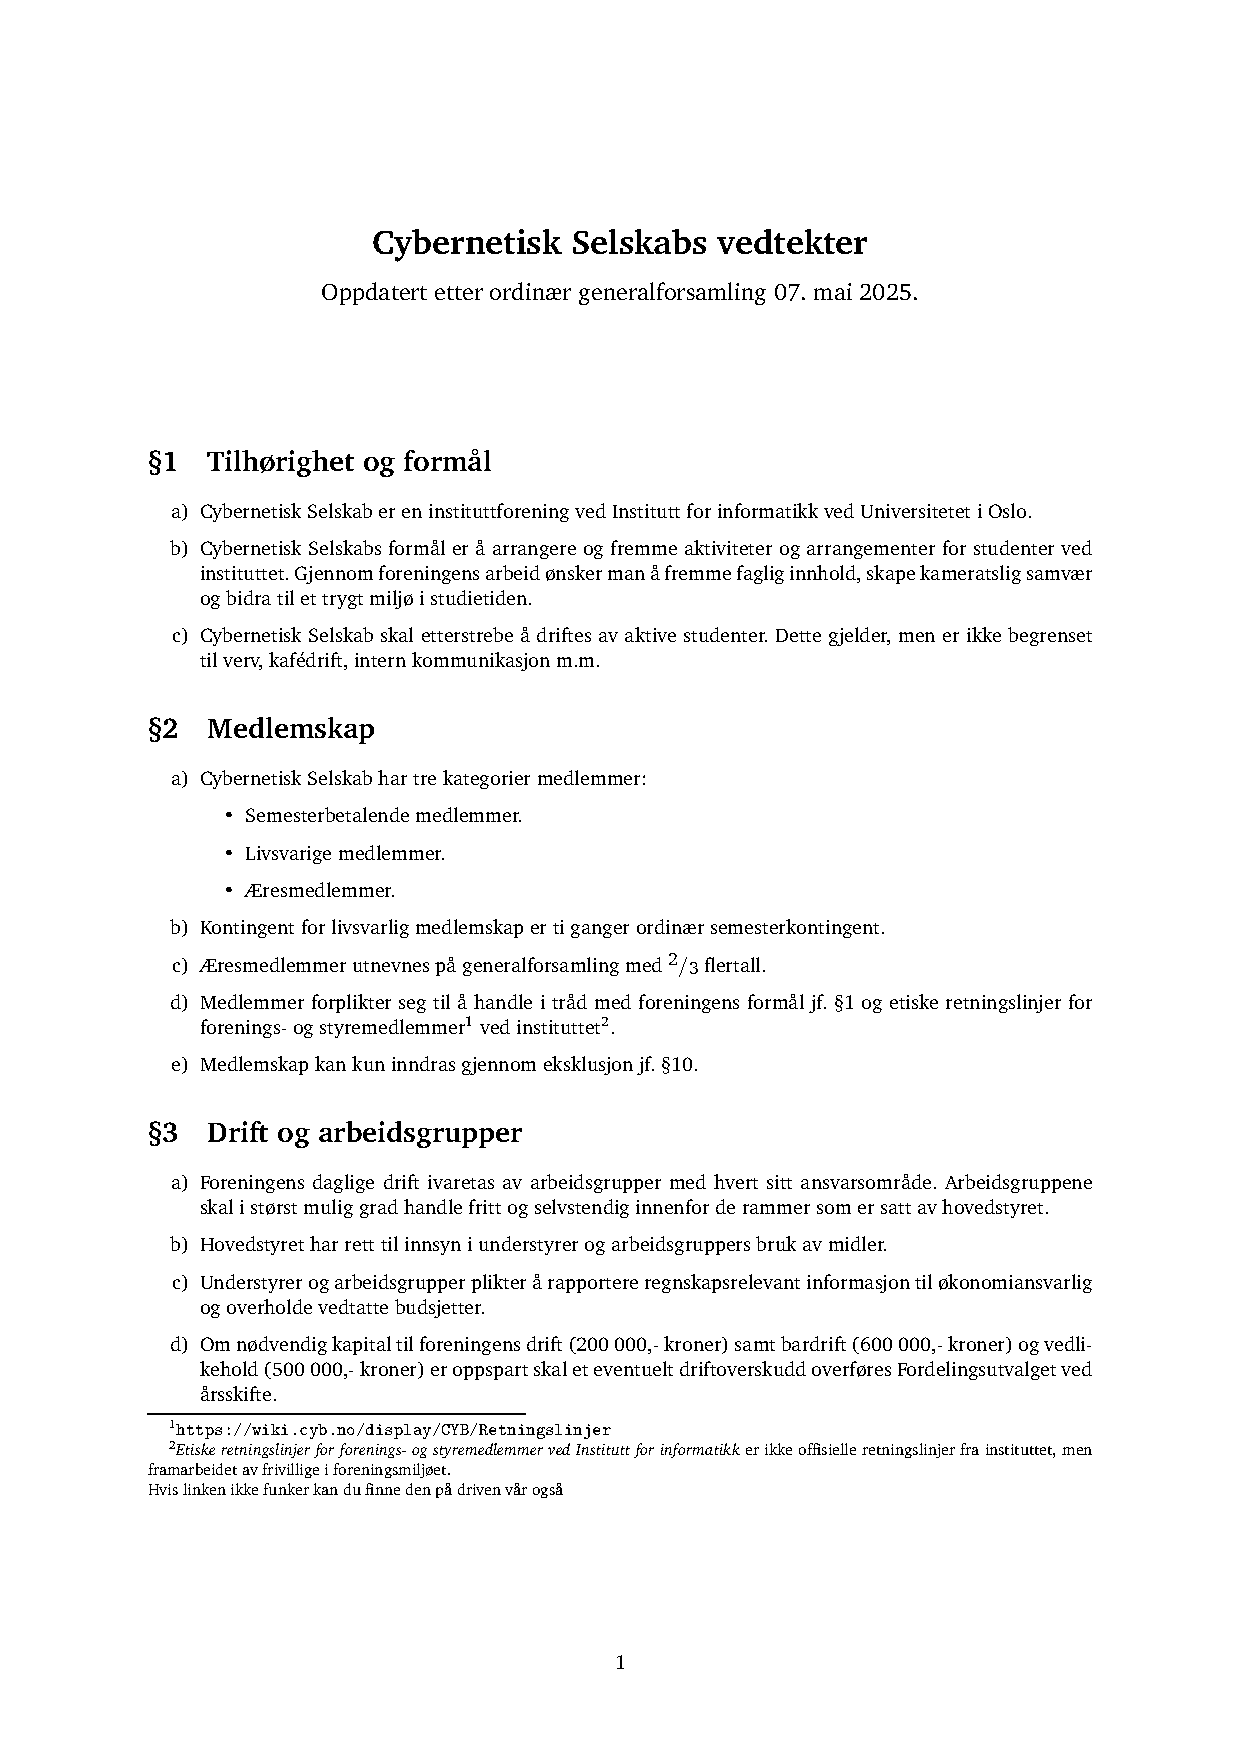
\includepdf[pages=-]{../vedtekter/vedtekter.pdf}

\end{document}
